\documentclass[tikz,border=10pt]{standalone}
\usepackage[utf8]{inputenc}
\usepackage[T1]{fontenc}
\usepackage{amsmath,amssymb}
\usepackage{tikz}
\usetikzlibrary{shapes.geometric, arrows.meta, positioning, calc, fit, backgrounds}

\definecolor{primary}{HTML}{0F172A}
\definecolor{primaryblue}{HTML}{1E3A8A}
\definecolor{accentblue}{HTML}{0284C7}
\definecolor{tealaccent}{HTML}{0D9488}
\definecolor{darkgreen}{HTML}{065F46}
\definecolor{lightgreen}{HTML}{ECFDF5}
\definecolor{crimson}{HTML}{991B1B}
\definecolor{lightred}{HTML}{FEF2F2}
\definecolor{amber}{HTML}{B45309}
\definecolor{lightamber}{HTML}{FFFBEB}
\definecolor{boxbg}{HTML}{F8FAFC}

\begin{document}

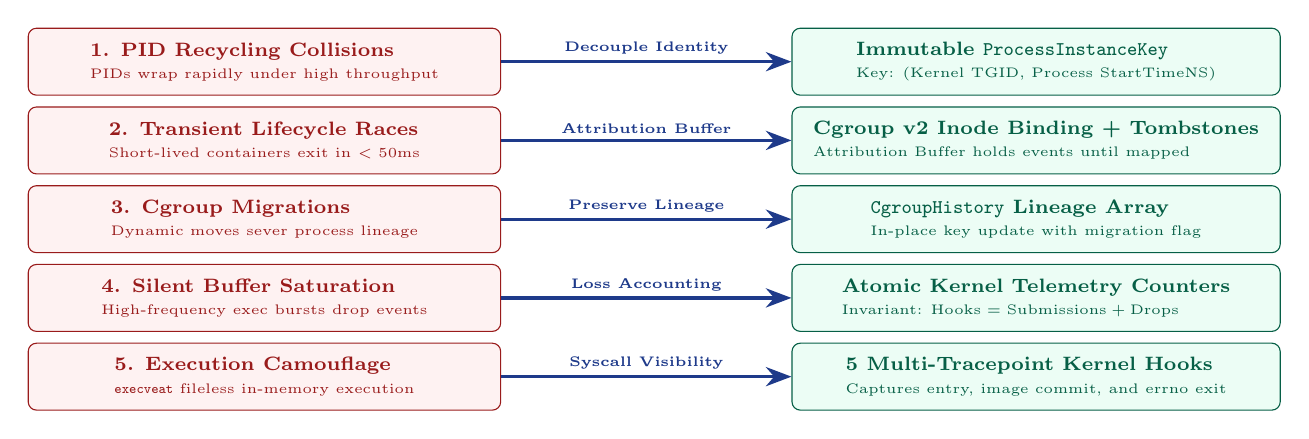
\begin{tikzpicture}[
    challenge/.style={rectangle, draw=crimson, fill=lightred, text=crimson, rounded corners=3pt, minimum width=6.0cm, minimum height=0.85cm, align=left, font=\scriptsize\bfseries},
    defense/.style={rectangle, draw=darkgreen, fill=lightgreen, text=darkgreen, rounded corners=3pt, minimum width=6.2cm, minimum height=0.85cm, align=left, font=\scriptsize\bfseries},
    conn/.style={-{Stealth[scale=1.1]}, very thick, draw=primaryblue}
]
    \node[challenge] (c1) at (0, 4.0) {1. PID Recycling Collisions\\ \tiny\textnormal{PIDs wrap rapidly under high throughput}};
    \node[challenge] (c2) at (0, 3.0) {2. Transient Lifecycle Races\\ \tiny\textnormal{Short-lived containers exit in $<50$ms}};
    \node[challenge] (c3) at (0, 2.0) {3. Cgroup Migrations\\ \tiny\textnormal{Dynamic moves sever process lineage}};
    \node[challenge] (c4) at (0, 1.0) {4. Silent Buffer Saturation\\ \tiny\textnormal{High-frequency exec bursts drop events}};
    \node[challenge] (c5) at (0, 0.0) {5. Execution Camouflage\\ \tiny\textnormal{\texttt{execveat} fileless in-memory execution}};

    \node[defense] (d1) at (9.8, 4.0) {Immutable \texttt{ProcessInstanceKey}\\ \tiny\textnormal{Key: (Kernel TGID, Process StartTimeNS)}};
    \node[defense] (d2) at (9.8, 3.0) {Cgroup v2 Inode Binding + Tombstones\\ \tiny\textnormal{Attribution Buffer holds events until mapped}};
    \node[defense] (d3) at (9.8, 2.0) {\texttt{CgroupHistory} Lineage Array\\ \tiny\textnormal{In-place key update with migration flag}};
    \node[defense] (d4) at (9.8, 1.0) {Atomic Kernel Telemetry Counters\\ \tiny\textnormal{Invariant: $\text{Hooks} = \text{Submissions} + \text{Drops}$}};
    \node[defense] (d5) at (9.8, 0.0) {5 Multi-Tracepoint Kernel Hooks\\ \tiny\textnormal{Captures entry, image commit, and errno exit}};

    \draw[conn] (c1.east) -- node[above, font=\tiny\bfseries\color{primaryblue}, inner sep=2pt]{Decouple Identity} (d1.west);
    \draw[conn] (c2.east) -- node[above, font=\tiny\bfseries\color{primaryblue}, inner sep=2pt]{Attribution Buffer} (d2.west);
    \draw[conn] (c3.east) -- node[above, font=\tiny\bfseries\color{primaryblue}, inner sep=2pt]{Preserve Lineage} (d3.west);
    \draw[conn] (c4.east) -- node[above, font=\tiny\bfseries\color{primaryblue}, inner sep=2pt]{Loss Accounting} (d4.west);
    \draw[conn] (c5.east) -- node[above, font=\tiny\bfseries\color{primaryblue}, inner sep=2pt]{Syscall Visibility} (d5.west);
\end{tikzpicture}

\end{document}
